% !TeX spellcheck = ru_RU
% !TEX root = vkr.tex

\section{Проектирование и реализация}
\label{sec:solution}

В результате реорганизации инфраструктура была приведена к единой структуре с точкой входа \texttt{main.py}, выделенными модулями в каталоге \texttt{src/}, единым конфигурационным файлом \texttt{matrices.yaml} и общими соглашениями по хранению промежуточных и итоговых данных. Архитектура реорганизованной инфраструктуры представлена на рисунке~\ref{fig:arch}.

\begin{figure}[h]
    \centering
    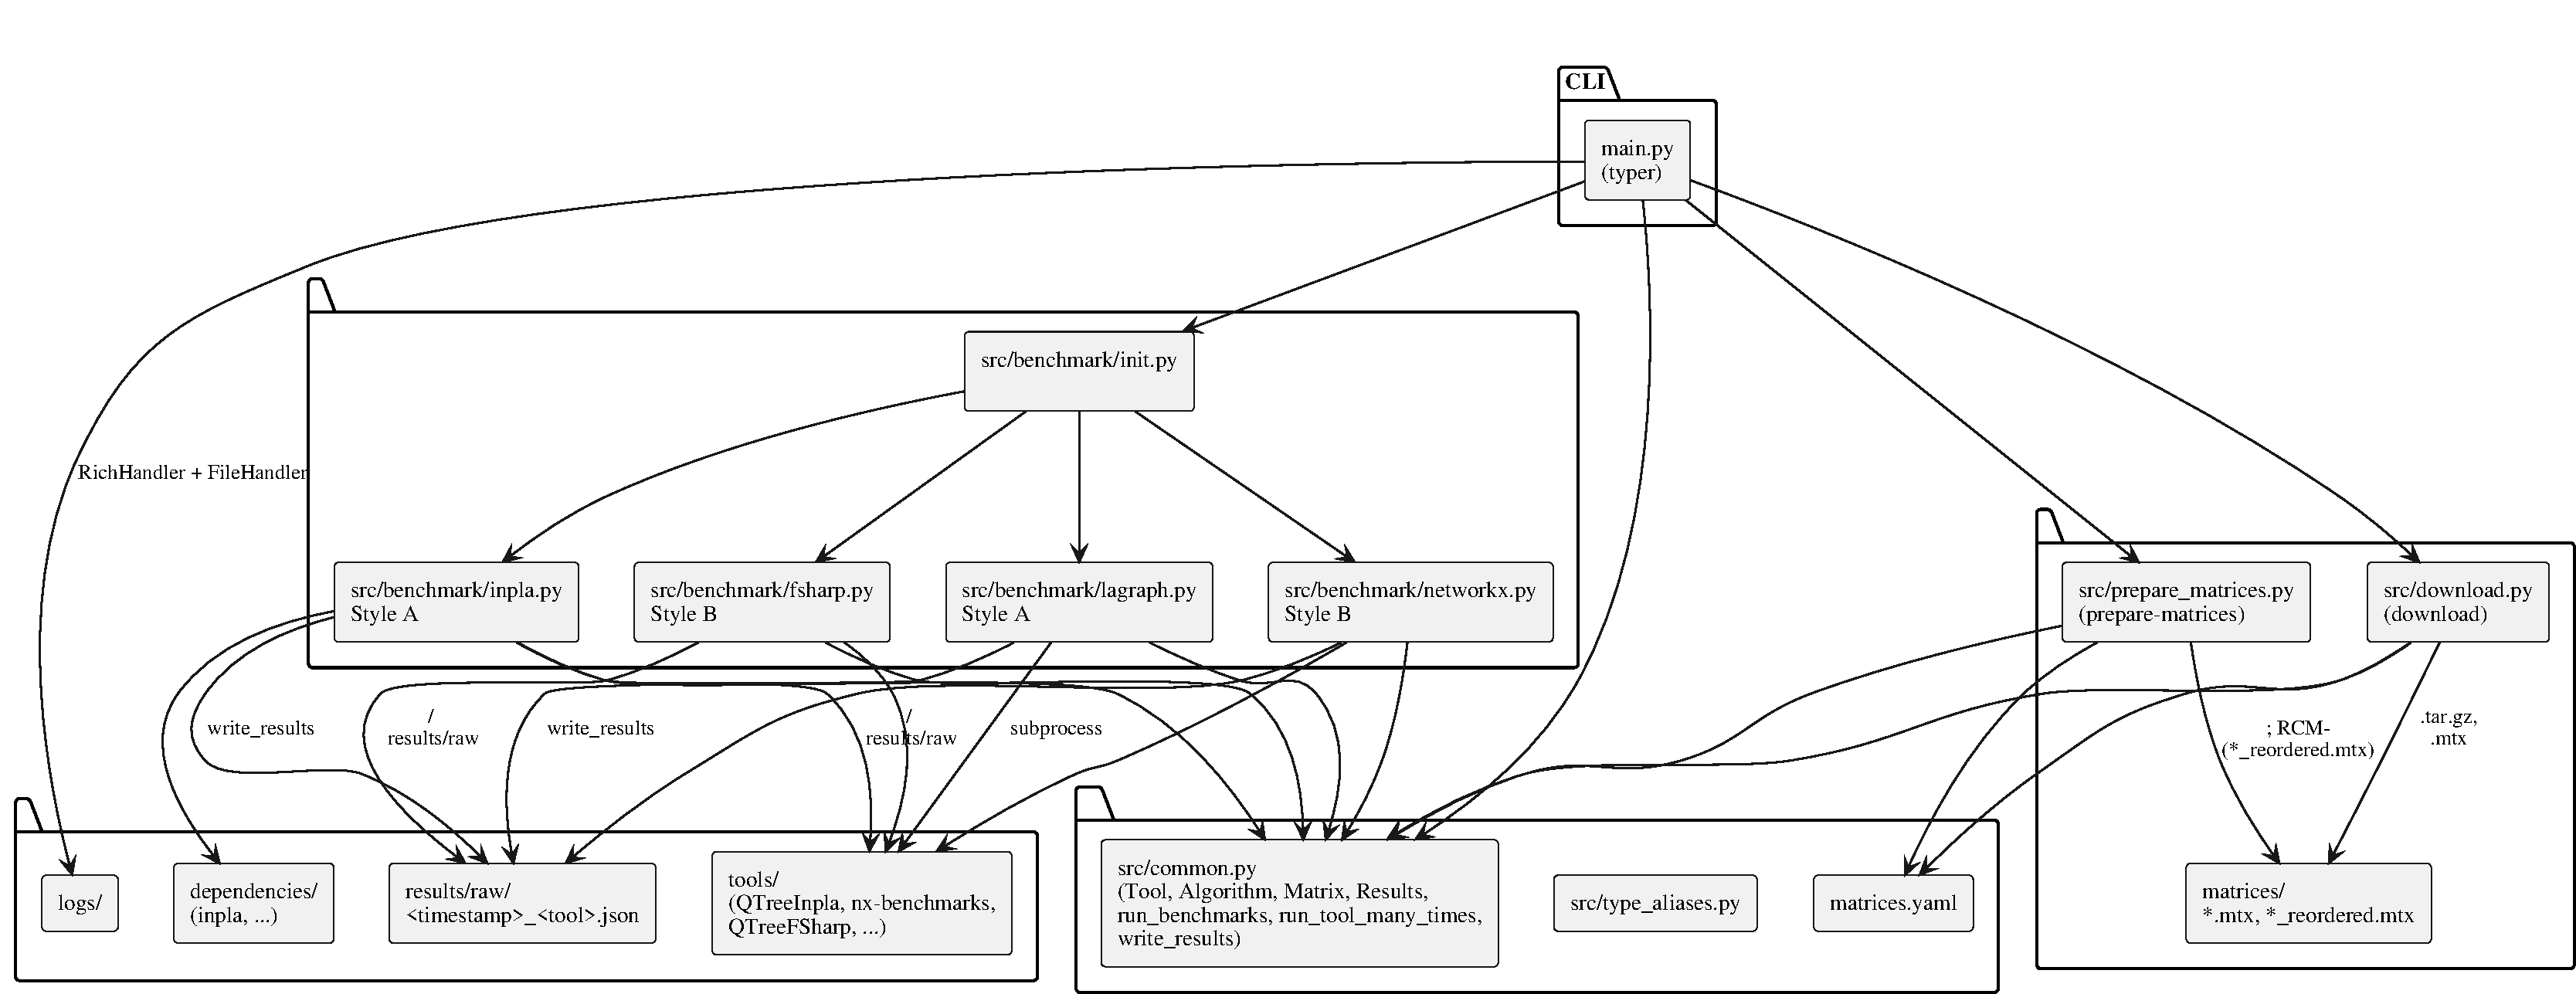
\includegraphics[width=\textwidth]{figures/arch.pdf}
    \caption{Архитектура реорганизованной инфраструктуры бенчмаркинга}
    \label{fig:arch}
\end{figure}

Поток данных при работе с инфраструктурой показан на рисунке~\ref{fig:pipeline}.

\begin{figure}[h]
    \centering
    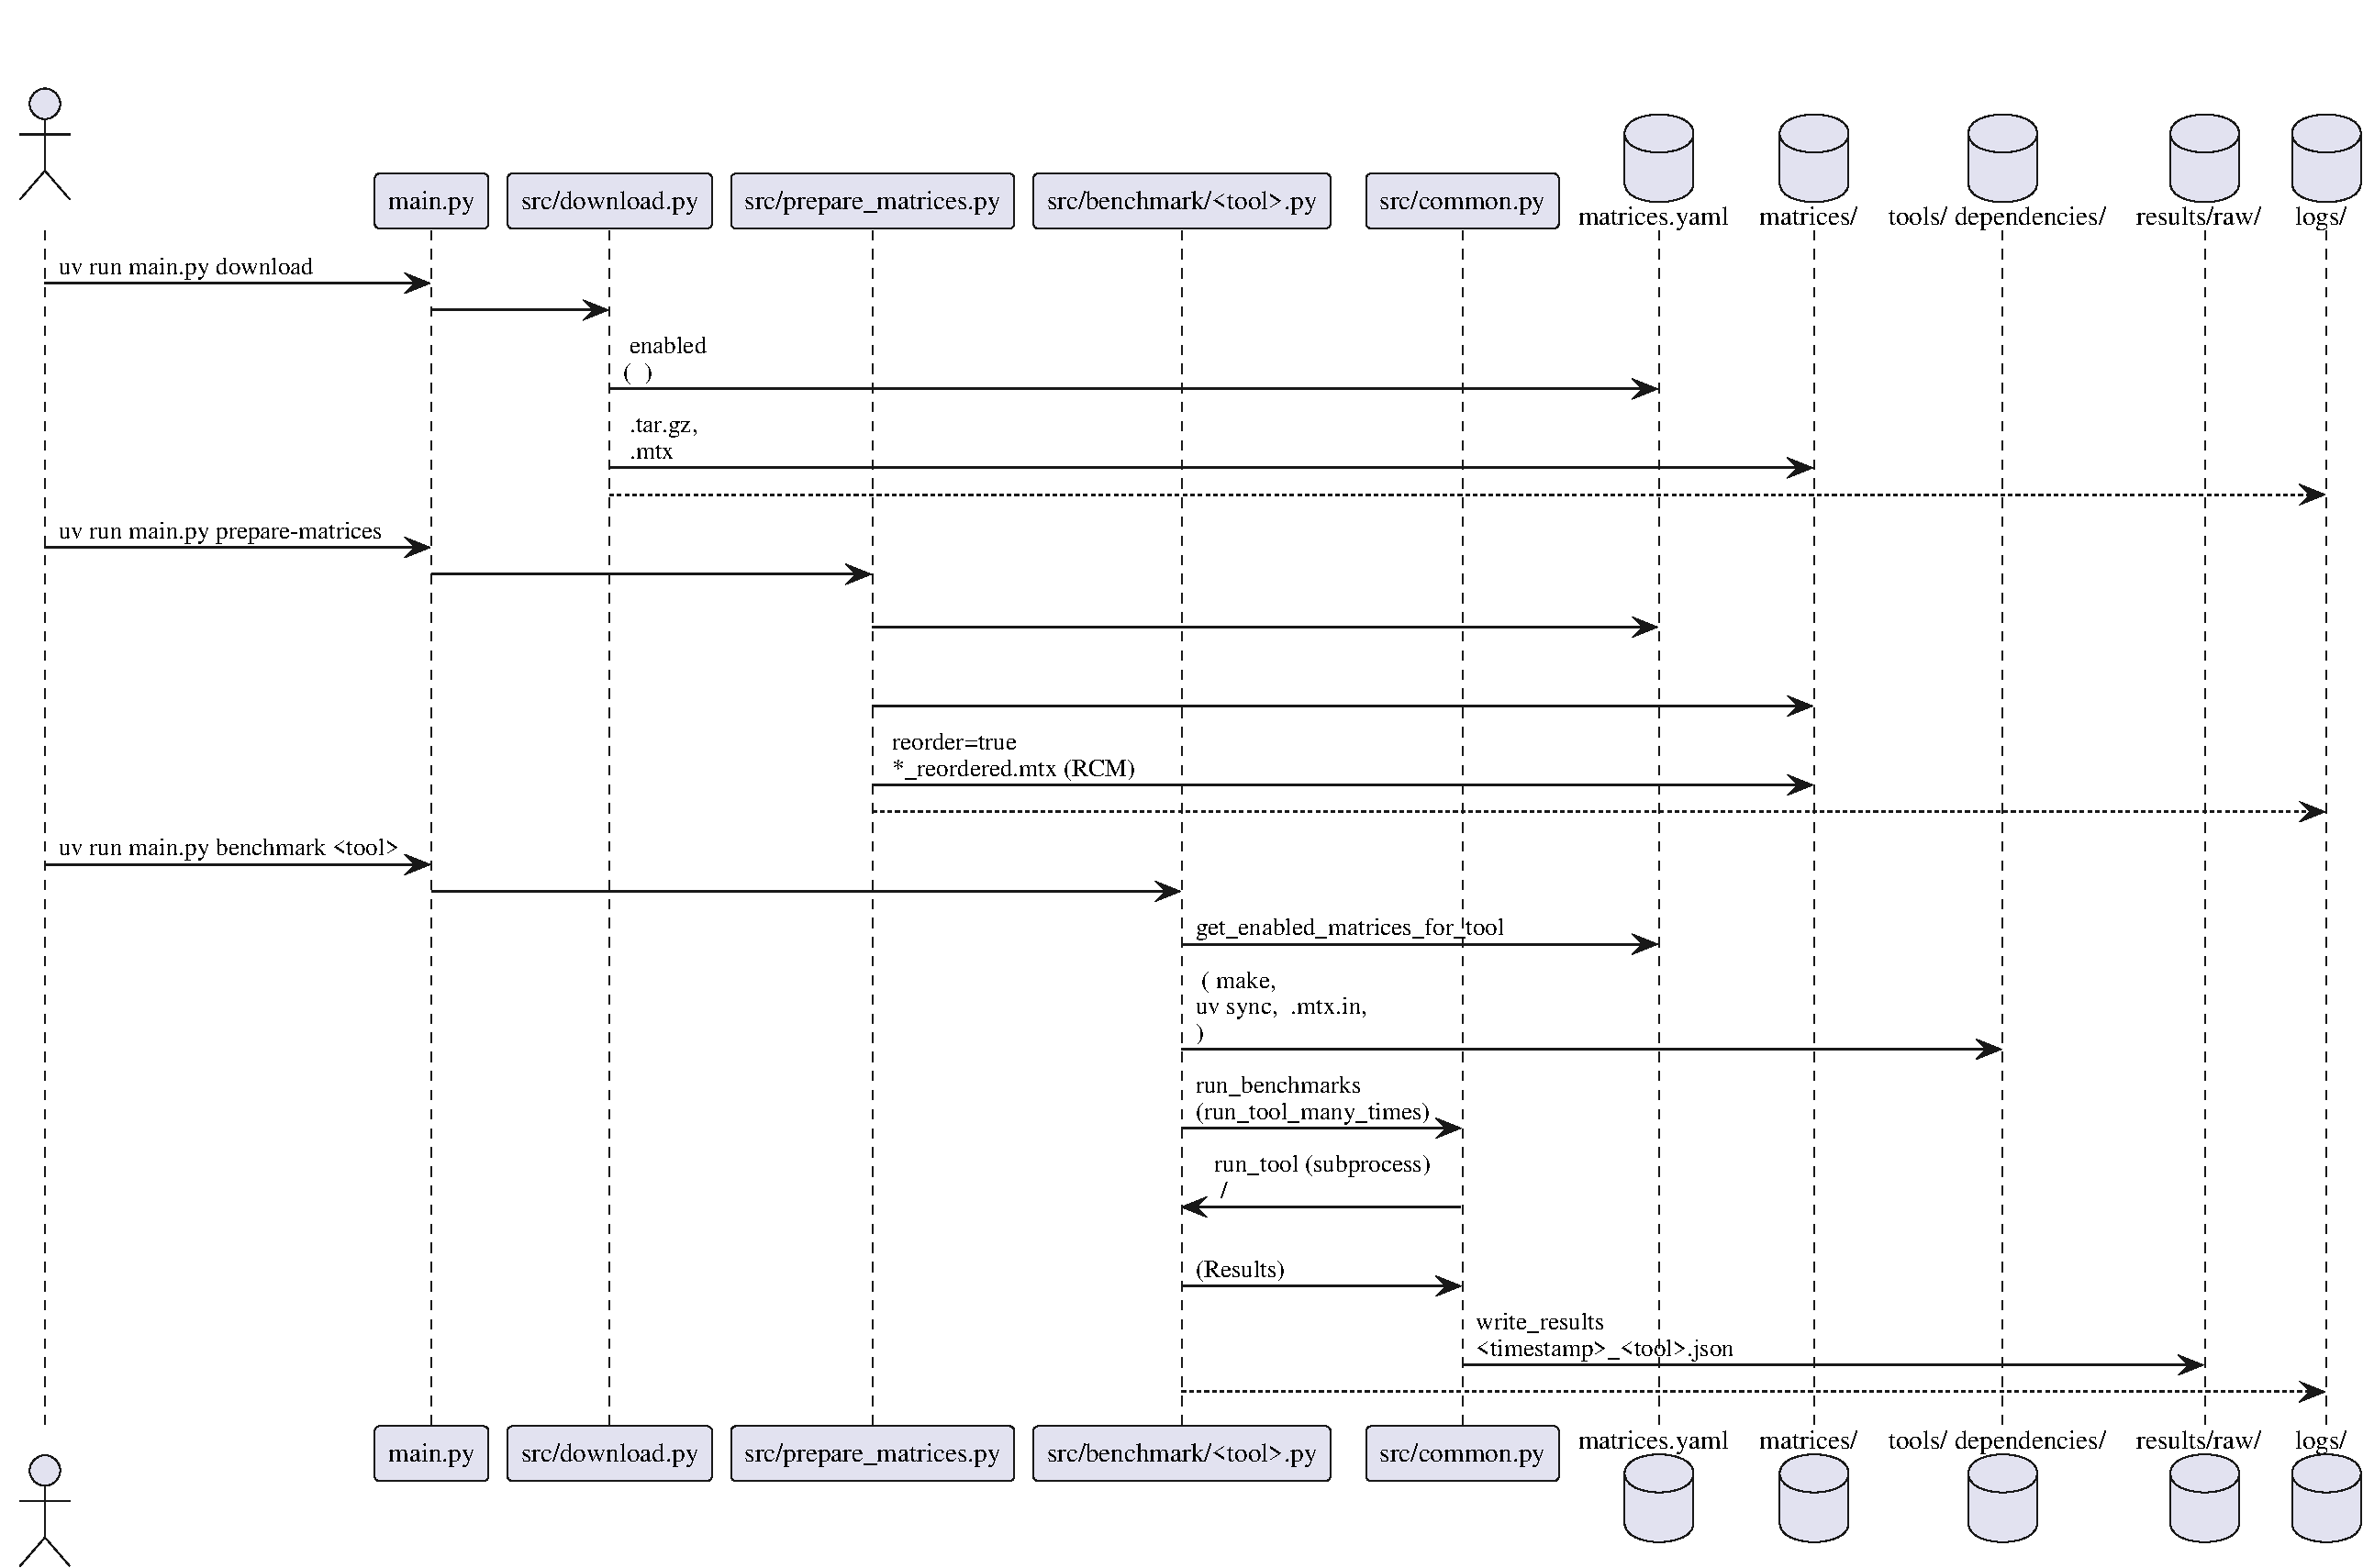
\includegraphics[width=\textwidth]{figures/pipeline.pdf}
    \caption{Поток данных инфраструктуры бенчмаркинга}
    \label{fig:pipeline}
\end{figure}

\subsection{Единый интерфейс командной строки}
\label{subsec:cli}

Точкой входа инфраструктуры является модуль \texttt{main.py}, реализованный с использованием библиотеки \texttt{typer}. CLI объединяет все этапы работы в виде подкоманд:

\begin{itemize}
    \item \texttt{download} --- загрузка и распаковка тестовых матриц;
    \item \texttt{prepare-matrices} --- предобработка матриц и построение переформированных версий;
    \item \texttt{benchmark <tool>} --- запуск бенчмаркинга для выбранного инструмента.
\end{itemize}

При старте приложения настраивается единое логирование: сообщения выводятся в консоль с использованием \texttt{RichHandler}, одновременно дублируясь в файл лога в каталоге \texttt{logs/} с временной меткой. Такой подход позволяет отслеживать ход выполнения эксперимента как в интерактивном режиме, так и при последующем анализе.

\subsection{Конфигурация и общие модули}
\label{subsec:common}

Вся конфигурация набора матриц, алгоритмов и инструментов хранится в файле \texttt{matrices.yaml}. Для загрузки и валидации используется модуль \texttt{src/common.py}, в котором определены:

\begin{itemize}
    \item перечисления \texttt{Tool} и \texttt{Algorithm} для типов инструментов и алгоритмов;
    \item структура \texttt{Matrix}, загружаемая из YAML при помощи \texttt{dataclass-wizard}, содержащая поля \texttt{name}, \texttt{enabled}, \texttt{algorithm}, \texttt{tools}, \texttt{reorder}, \texttt{link};
    \item тип \texttt{Results} в виде словаря, отражающий единый формат хранения результатов: для каждого алгоритма (\texttt{bfs}, \texttt{sssp}, \texttt{tc}) отображение базового имени матрицы в отображение числа потоков (в виде строки) в список строк вывода за каждый прогон.
\end{itemize}

В \texttt{src/common.py} вынесены общие утилиты: функции для выбора включённых матриц с фильтрацией по инструменту, построения базового имени матрицы и имён файлов, функции \texttt{run\_tool\_many\_times} и \texttt{run\_benchmarks} для организации измерений по числу потоков и количеству прогонов, а также функция \texttt{write\_results}, сохраняющая результаты в файл вида \texttt{results/raw/<timestamp>\_<tool>.json}. Единое именование файлов обеспечивает совместимость с кодом построения графиков.

\subsection{Загрузка и подготовка матриц}
\label{subsec:download}

Загрузка матриц реализована в модуле \texttt{src/download.py}. Команда \texttt{download} считывает из \texttt{matrices.yaml} список включённых матриц, убирает дубли по имени при помощи \texttt{get\_unique\_by\_name\_matrices}, скачивает архивы по ссылкам, распаковывает их и копирует файлы \texttt{.mtx} в каталог \texttt{matrices/}. Если файл матрицы уже существует, загрузка пропускается.

Предобработка матриц реализована в модуле \texttt{src/prepare\_matrices.py}. Команда \texttt{prepare-matrices} выполняет два этапа:

\begin{enumerate}
    \item Приведение матрицы к виду с неотрицательными целыми элементами. При наличии отрицательных элементов значение минимального элемента добавляется ко всем элементам, после чего вызывается \texttt{eliminate\_zeros()}.
    \item Для матриц с флагом \texttt{reorder: true} строится переформированная версия с использованием алгоритма обратного алгоритма Катхилла--Макки (\emph{Reverse Cuthill--McKee}, RCM). При этом строится симметризованная бинарная матрица для вычисления перестановки, удаляются диагональные элементы, перестановка применяется к исходной матрице; для прямоугольных матриц переставляются только строки. Результат сохраняется с суффиксом \texttt{\_reordered.mtx}.
\end{enumerate}

\subsection{Интеграция инструментов}
\label{subsec:integration}

Все модули интеграции инструментов размещены в каталоге \texttt{src/benchmark/}. Регистрация подкоманд осуществляется в \texttt{src/benchmark/\_\_init\_\_.py} через \texttt{app.add\_typer()}. В инфраструктуре выделены два стиля интеграции.

\subsubsection{Стиль A: subprocess и парсинг stdout}
Стиль A используется для инструментов, непосредственно выводящих времена работы в стандартный вывод. К данному стилю относятся \texttt{lagraph} и \texttt{inpla}. Для них определяется функция-\texttt{runner}, принимающая объект \texttt{Matrix} и число потоков и возвращающая \texttt{subprocess.CompletedProcess[str]}. Общий цикл измерений, повторений и агрегации по числу потоков делегируется функциям \texttt{run\_benchmarks}/\texttt{run\_tool\_many\_times} из \texttt{src/common.py}, после чего результаты сохраняются через \texttt{write\_results}.

\subsubsection{Стиль B: пользовательский сборщик результатов}
Стиль B применяется, когда инструмент использует собственный фреймворк для запуска бенчмарков и формирует собственный отчёт. К данному стилю относятся \texttt{networkx} и \texttt{fsharp}. В этом случае модуль бенчмарка отвечает за подготовку окружения (например, \texttt{uv sync}), очистку и создание символьных ссылок на матрицы, запуск harness'а инструмента, поиск последнего сформированного JSON-отчёта и копирование его в \texttt{results/raw/} с единым именованием.

\subsubsection{Особенности интеграции Inpla}
\label{subsec:inpla}

Интеграция \texttt{Inpla}/\texttt{QTreeInpla} имеет ряд специфичных особенностей:

\begin{itemize}
    \item \textbf{Сборка.} Перед запуском бенчмарков выполняется сборка интерпретатора \texttt{Inpla} из каталога \texttt{dependencies/inpla} при помощи \texttt{make} (последовательность \texttt{make clean}, \texttt{make}, \texttt{make clean}, \texttt{make thread}).
    \item \textbf{Проверка.} При указании флага \texttt{--check} запускается тестовый скрипт \texttt{test.fsx} из каталога \texttt{tools/QTreeInpla} для верификации работоспособности сборки.
    \item \textbf{Конвертация матриц.} Матрицы из формата \texttt{.mtx} конвертируются в формат \texttt{.in}, используемый \texttt{QTreeInpla}, при помощи скрипта \texttt{scripts/mtx\_to\_experiment.fsx} в каталоге \texttt{tools/QTreeInpla}. Конвертированные файлы размещаются в подкаталогах вида \texttt{experiments\_<algorithm>/}.
    \item \textbf{Запуск.} Для каждого измерения вызывается исполняемый файл \texttt{inpla} с параметрами \texttt{-t <thread\_count>}, \texttt{-f <path>} и \texttt{-Xms <memory>}. Число потоков задаётся явно, объём памяти на запуск рассчитывается пропорционально числу потоков с учётом параметра \texttt{memory\_limit\_for\_1\_thread}.
    \item \textbf{Ограничения окружения.} При запуске устанавливается неограниченный лимит стека (\texttt{RLIMIT\_STACK}) для избежания переполнения стека при больших матрицах. Код возврата процесса не считается фатальным (\texttt{check=False}), так как \texttt{Inpla} в некоторых случаях может завершаться с ненулевым кодом, при этом сохраняя вывод, необходимый для анализа.
\end{itemize}

\subsection{Расширяемость инфраструктуры}
\label{subsec:extensibility}

Для упрощения добавления новых инструментов в инфраструктуре формализован процесс расширения, описанный в \texttt{EXTENDING.md}. Процесс включает следующие шаги:

\begin{enumerate}
    \item Добавить вариант в перечисление \texttt{Tool} в \texttt{src/common.py}.
    \item Создать модуль \texttt{src/benchmark/<tool>.py} с реализацией по одному из стилей интеграции, используя общие опции и утилиты из \texttt{src/common.py} и \texttt{src/type\_aliases.py}.
    \item Зарегистрировать приложение в \texttt{src/benchmark/\_\_init\_\_.py}.
    \item Добавить инструмент в список \texttt{tools} соответствующих записей в \texttt{matrices.yaml}.
    \item Сохранять результаты исключительно через \texttt{write\_results} для соблюдения соглашения об именовании файлов.
\end{enumerate}

Также в инфраструктуре предусмотрены соглашения по размещению кода: репозитории инструментов добавляются в \texttt{tools/}, зависимости (например, интерпретаторы или библиотеки) --- в \texttt{dependencies/} в виде подмодулей \texttt{git}. Документация для разработчиков приведена в \texttt{AGENTS.md} и \texttt{EXTENDING.md}.
